\section{TÌM HIỂU VÀ KHAI THÁC DỊCH VỤ ĐIỆN TOÁN ĐÁM MÂY ORACLE CLOUD}
\subsection{Giới thiệu tổng quan về (Oracle Cloud Infrastructure – OCI)}
Oracle Cloud Infrastructure (OCI) là nền tảng IaaS (Infrastructure as a Service) của Oracle, được thiết kế để chạy mọi loại ứng dụng – từ ứng dụng doanh nghiệp truyền thống đến các ứng dụng đám mây hiện đại – với hiệu suất cao hơn, bảo mật tốt hơn và chi phí tối ưu hơn so với nhiều giải pháp khác.

Đặc điểm nổi bật

\begin{myitem}
\item Hiệu năng và tốc độ cao

  \begin{mysubitem}
    \item Oracle Cloud Infrastructure (OCI) nổi bật nhờ cung cấp hạ tầng phần cứng hiện đại, được tối ưu để đáp ứng nhu cầu xử lý khối lượng công việc lớn. Các máy chủ trong OCI sử dụng công nghệ mới nhất, đảm bảo khả năng tính toán mạnh mẽ và ổn định. Hệ thống mạng có độ trễ cực thấp, giúp ứng dụng doanh nghiệp có thể phản hồi nhanh chóng, ngay cả trong những tác vụ yêu cầu xử lý theo thời gian thực. Điều này mang lại trải nghiệm tốt cho người dùng cuối cũng như tối ưu hóa hiệu quả vận hành cho doanh nghiệp.
    
    \item Ngoài ra, kiến trúc của OCI được thiết kế theo hướng tối ưu hóa hiệu suất. Các dịch vụ đều có khả năng mở rộng linh hoạt, hỗ trợ doanh nghiệp tăng hoặc giảm tài nguyên tính toán chỉ trong vài phút. Nhờ vậy, hệ thống luôn duy trì tốc độ cao mà không bị gián đoạn, đồng thời giúp doanh nghiệp dễ dàng đáp ứng những biến động bất ngờ về nhu cầu sử dụng.

  \end{mysubitem}

\item Bảo mật và an toàn dữ liệu

  \begin{mysubitem}
    \item Một trong những thế mạnh lớn nhất của OCI chính là bảo mật. Hệ thống được xây dựng với nhiều lớp phòng thủ, bao gồm bảo mật ở cấp hạ tầng vật lý, cấp mạng, cũng như cấp ứng dụng. Điều này giúp bảo vệ dữ liệu và dịch vụ trước các nguy cơ tấn công từ bên ngoài cũng như rủi ro nội bộ.
    
    \item Bên cạnh đó, Oracle đã tích hợp sẵn nhiều tính năng bảo mật tự động như mã hóa dữ liệu (Data Encryption), quản lý danh tính và truy cập (Identity \& Access Management - IAM), cùng với các công cụ tường lửa và Security Lists. Nhờ vậy, ngay cả khi không có đội ngũ chuyên gia bảo mật chuyên sâu, doanh nghiệp vẫn có thể duy trì mức độ an toàn dữ liệu cao, giảm thiểu rủi ro rò rỉ hoặc thất thoát thông tin.
    
  \end{mysubitem}

\item Hỗ trợ cơ sở dữ liệu tự động (Autonomous Database)

  \begin{mysubitem}
    \item Autonomous Database được xem là điểm nhấn quan trọng và khác biệt nhất của OCI. Đây là dịch vụ cơ sở dữ liệu thông minh, có khả năng tự động hóa gần như toàn bộ quy trình quản trị như vá lỗi hệ thống, sao lưu dữ liệu, tối ưu hiệu suất, hay thậm chí tự động mở rộng khi cần thiết. Doanh nghiệp sẽ không phải lo lắng về những công việc phức tạp thường tốn rất nhiều nhân lực quản trị truyền thống.
    
    \item Sự tự động này không chỉ giúp giảm chi phí vận hành mà còn hạn chế tối đa rủi ro do lỗi con người. Dữ liệu quan trọng được bảo vệ tốt hơn, luôn trong trạng thái sẵn sàng và có hiệu năng cao nhất. Điều này đặc biệt phù hợp với các tổ chức, doanh nghiệp cần hệ thống cơ sở dữ liệu hoạt động liên tục và ổn định 24/7.
    
  \end{mysubitem}

\item Chi phí hợp lý

  \begin{mysubitem}
    \item Một trong những rào cản lớn của doanh nghiệp khi chuyển đổi sang nền tảng đám mây chính là chi phí. Tuy nhiên, Oracle đã giải quyết vấn đề này bằng cách đưa ra mô hình định giá minh bạch và cạnh tranh. Người dùng có thể lựa chọn gói thanh toán theo mức độ sử dụng (pay-as-you-go) hoặc đăng ký theo gói dài hạn (subscription), tùy theo nhu cầu cụ thể của mình.
    
    \item Nhờ cơ chế này, doanh nghiệp dễ dàng dự đoán và kiểm soát ngân sách, không còn phải lo chi phí phát sinh bất ngờ. Quan trọng hơn, mô hình chi phí linh hoạt còn giúp doanh nghiệp mở rộng hệ thống mà không cần đầu tư lớn vào hạ tầng vật lý, từ đó giảm tải áp lực tài chính và nâng cao hiệu quả sử dụng vốn.
    
  \end{mysubitem}

\item Dịch vụ đa dạng và tự động hóa

  \begin{mysubitem}
    \item Oracle Cloud không chỉ dừng lại ở Compute hay Database, mà còn cung cấp một hệ sinh thái phong phú với nhiều dịch vụ khác như lưu trữ (Storage), mạng (Networking), bảo mật (Security), container, trí tuệ nhân tạo (AI/ML), phân tích dữ liệu (Analytics), và nhiều công cụ phục vụ doanh nghiệp trong kỷ nguyên số. Sự đa dạng này cho phép tổ chức triển khai hầu hết mọi ứng dụng và dịch vụ ngay trên cùng một nền tảng.
    
    \item Ngoài ra, OCI hỗ trợ tích hợp API, SDK, cùng các công cụ quản lý tự động, giúp người dùng dễ dàng triển khai, giám sát và tối ưu hệ thống. Điều này không chỉ tiết kiệm thời gian vận hành mà còn giảm gánh nặng cho đội ngũ kỹ thuật. Với khả năng tự động hóa cao, doanh nghiệp có thể tập trung nhiều hơn vào các hoạt động cốt lõi thay vì phải tốn nhiều công sức duy trì hạ tầng.
    
  \end{mysubitem}

\end{myitem}

\subsection{Đăng ký và đăng nhập}
\subsubsection{Đăng ký}

\textit{Chú ý: chúng ta cần phải có Thẻ tín dụng quốc tế để đăng ký tài khoản. Oracle sẽ xác nhận thẻ bằng cách charge 1.38SGD khi đăng ký và sẽ hoàn lại ngay sau đó.}

\begin{myitem}
\item Bước 1: Truy cập vào trang https://www.oracle.com/cloud/free/ và nhấn vào Start for free.

\begin{figure}[H] % cần gói float nếu muốn fix vị trí
    \centering
    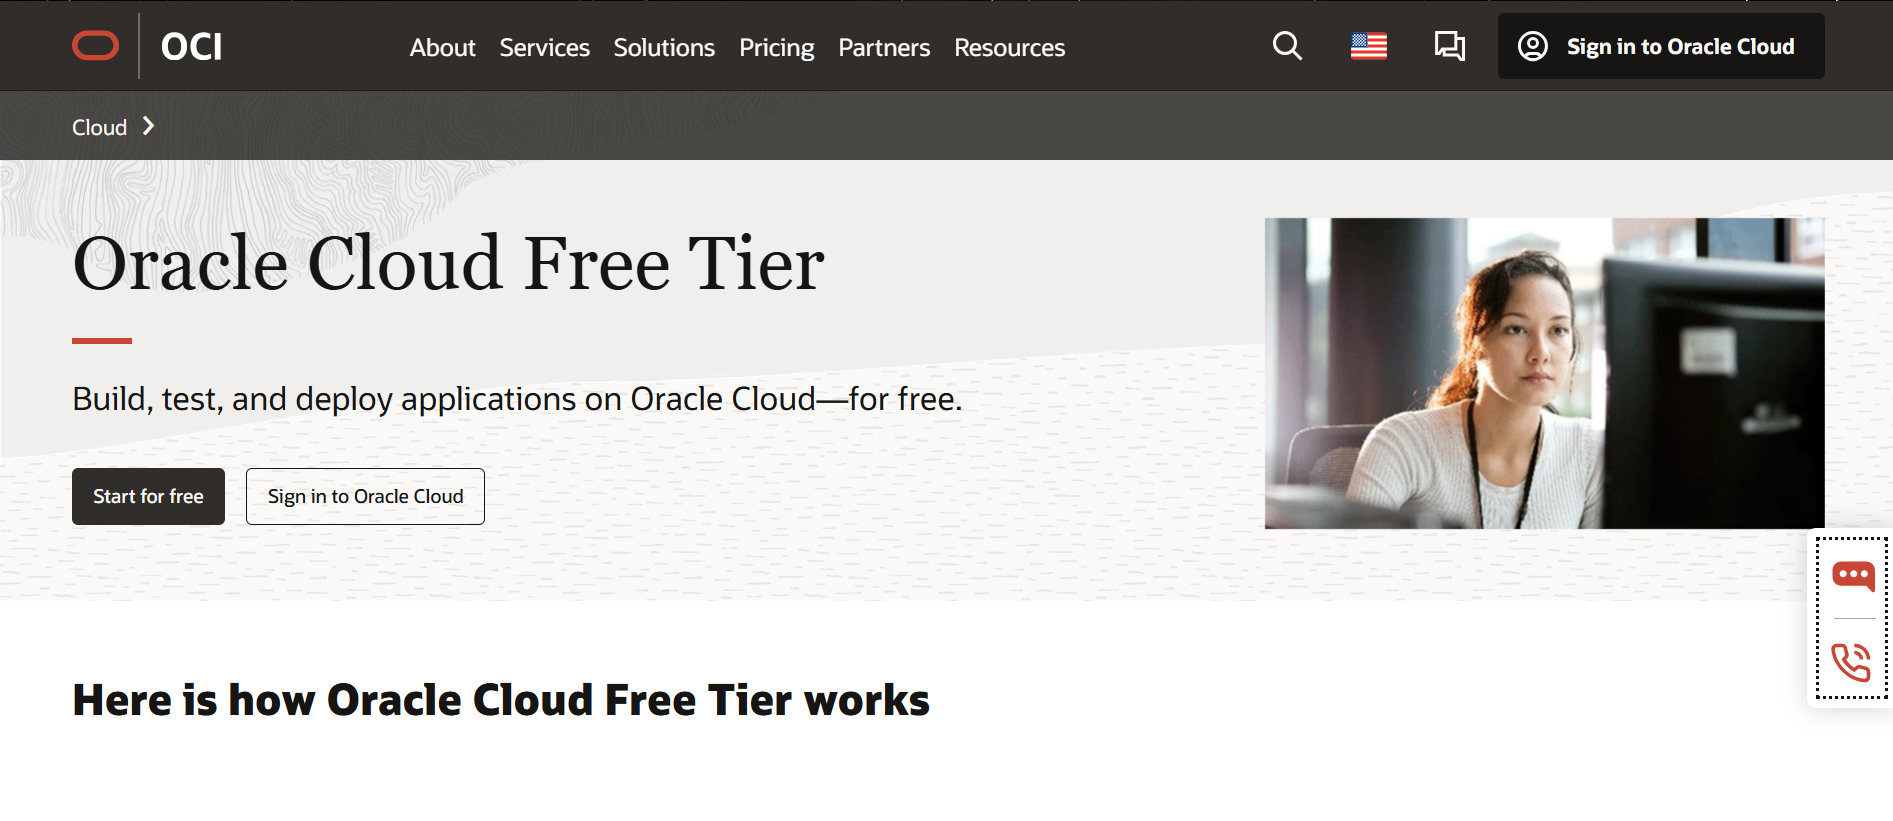
\includegraphics[width=0.7\textwidth]{Demo/Giao_dien_truy_cap.png}
    \caption{Giao diện khi truy cập vào trang web OCI}
    \label{fig:cloud_intro}
\end{figure}

\item Bước 2: Điền thông tin cơ bản của người dùng và nhấn Verity my email để tiếp tục.

\begin{figure}[H] % cần gói float nếu muốn fix vị trí
    \centering
    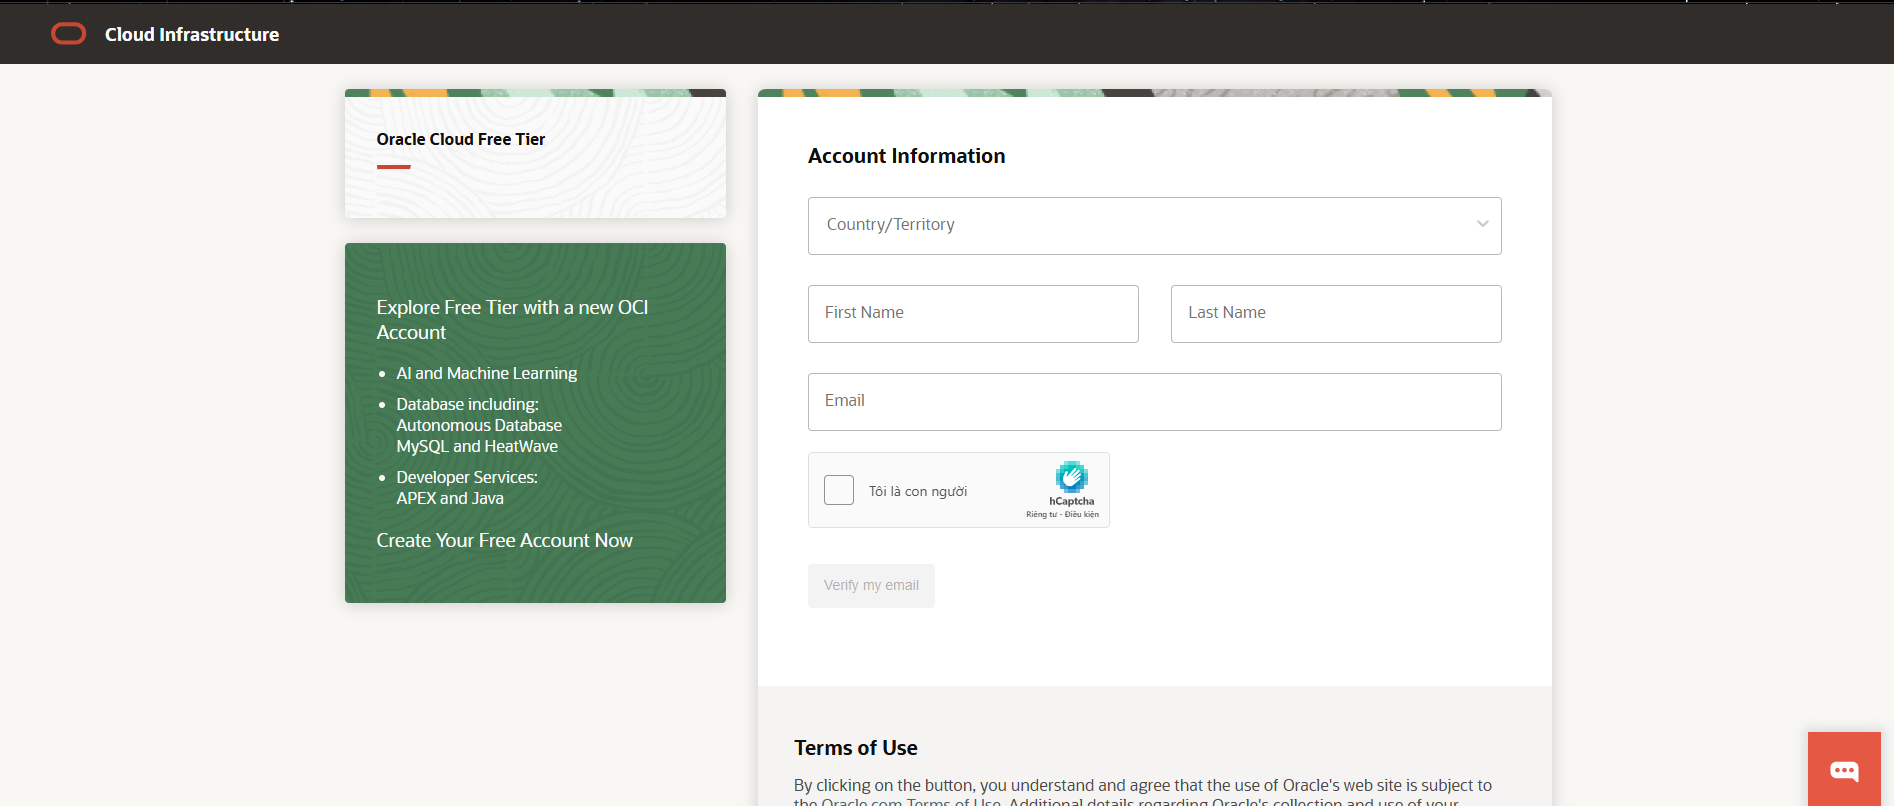
\includegraphics[width=0.9\textwidth]{Demo/Account_Information.png}
    \caption{Giao diện Account Information điền thông tin cơ bản}
    \label{fig:cloud_intro}
\end{figure}

\item Bước 3: Điền các thông tin về tài khoản đăng nhập vào các ô để tiếp tục.

\begin{figure}[H] % cần gói float nếu muốn fix vị trí
    \centering
    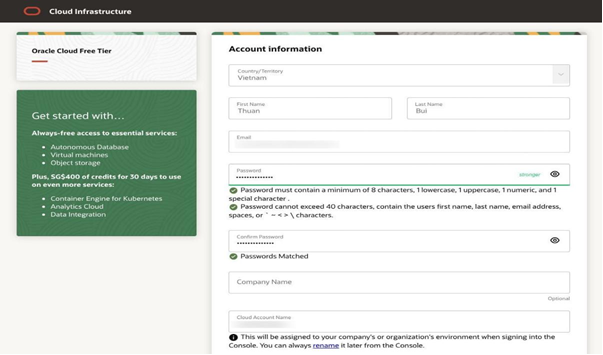
\includegraphics[width=0.9\textwidth]{Demo/Account_Information_dang_nhap.png}
    \caption{Giao diện Account Information điền các thông tin đăng nhập}
    \label{fig:cloud_intro}
\end{figure}

\item Bước 4: Nhập thông tin cá nhân: Địa chỉ (Address),Điện thoại (Phone Number) và Payment verification.

\begin{figure}[H] % cần gói float nếu muốn fix vị trí
    \centering
    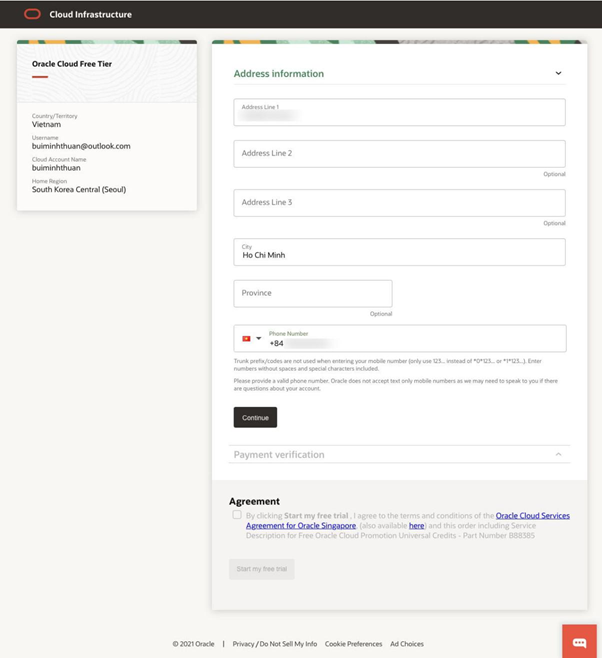
\includegraphics[width=0.7\textwidth]{Demo/Address_Information.png}
    \caption{Giao diện Address Information}
    \label{fig:cloud_intro}
\end{figure}

\item Bước 5: Bấm Continue, đợi hệ thống xử lý và hoàn tất quá trình tạo tài khoản.

\begin{figure}[H] % cần gói float nếu muốn fix vị trí
    \centering
    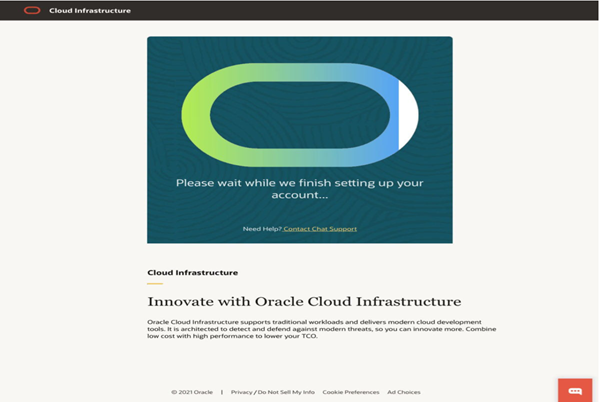
\includegraphics[width=0.7\textwidth]{Demo/Cho_doi_hoan_tat.png}
    \caption{Giao diện chờ đợi quá trình hoàn tất tạo tài khoản.}
    \label{fig:cloud_intro}
\end{figure}

\end{myitem}

\subsubsection{Đăng nhập}
\begin{myitem}
\item Bước 1: Tiến hành truy cập theo vào trang https://www.oracle.com/cloud/sign-in.html và nhập điền tên tài khoản đăng nhập vào Cloud Account Name.

\begin{figure}[H] % cần gói float nếu muốn fix vị trí
    \centering
    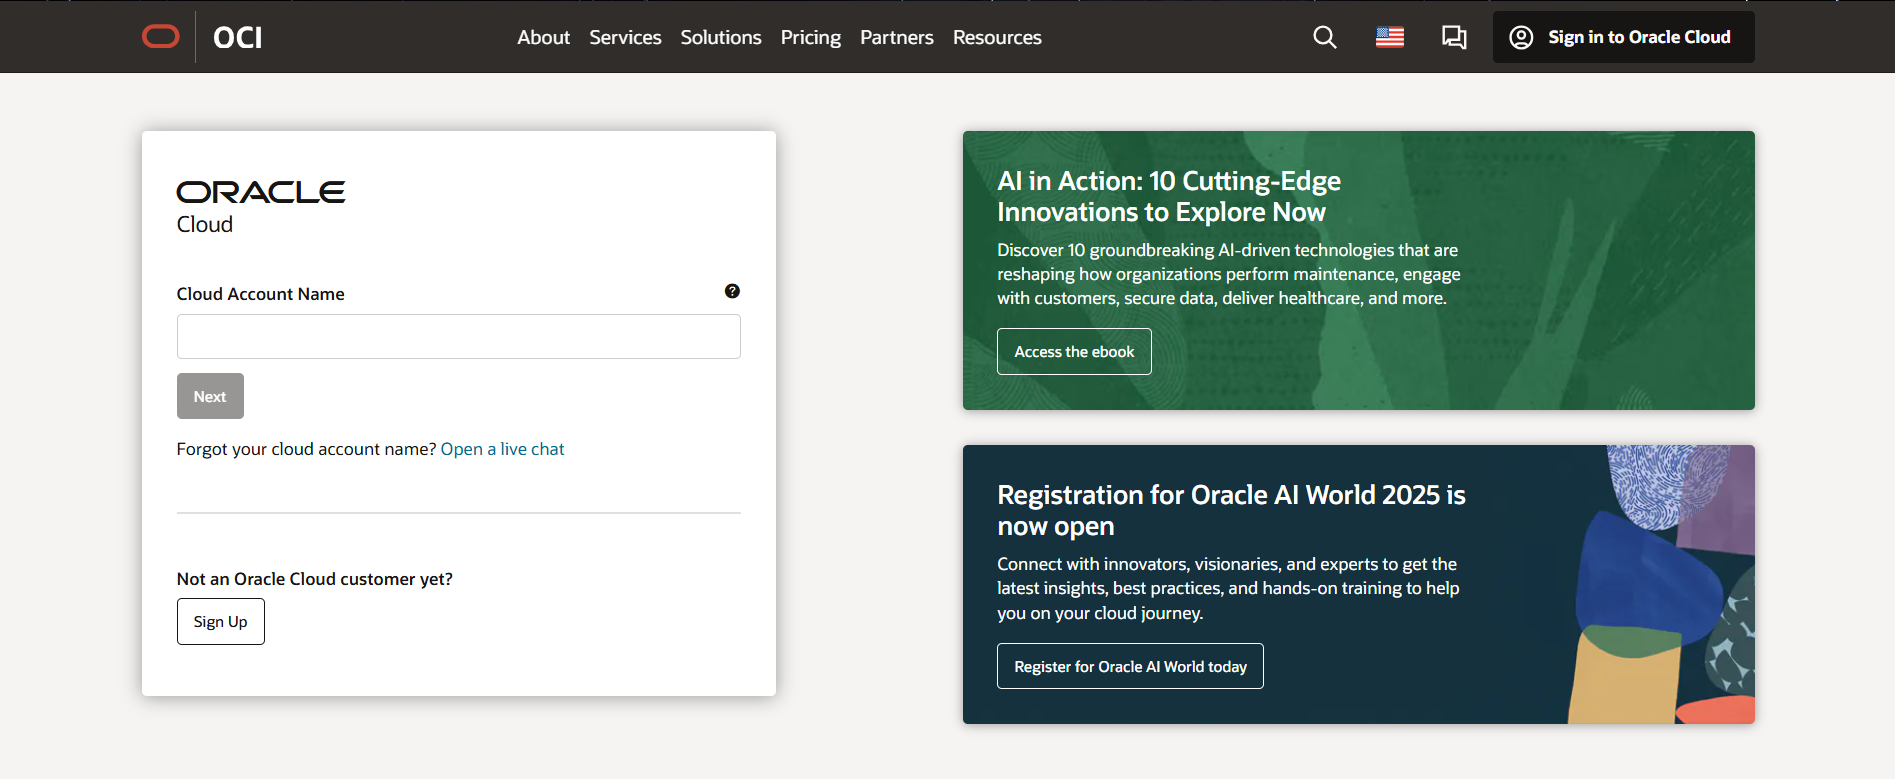
\includegraphics[width=0.9\textwidth]{Demo/Trang_dang_nhap.png}
    \caption{Giao diện trang đăng nhập tài khoản}
    \label{fig:cloud_intro}
\end{figure}

\item Bước 2: Nhập tiếp email của chúng ta vào ô User Name và mật khẩu vào ô Password.

\begin{figure}[H] % cần gói float nếu muốn fix vị trí
    \centering
    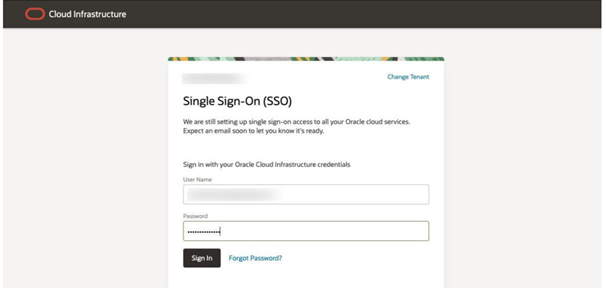
\includegraphics[width=0.9\textwidth]{Demo/Single_Sign_On.png}
    \caption{Giao diện Single Sign-On (SSO)}
    \label{fig:cloud_intro}
\end{figure}

\item Bước 3: Nhấn Sign In, đăng nhập thành công vào Dashboard của Oracle Cloud.

\begin{figure}[H] % cần gói float nếu muốn fix vị trí
    \centering
    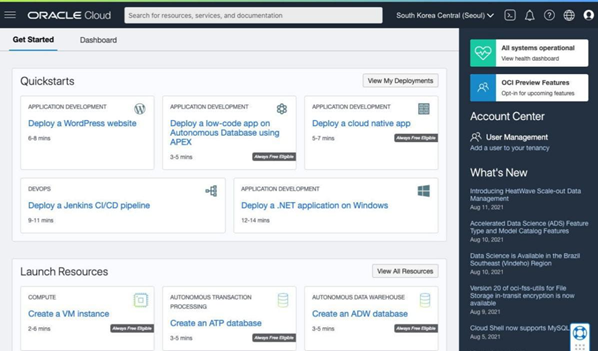
\includegraphics[width=0.9\textwidth]{Demo/Dang_nhap_thanh_cong.png}
    \caption{Giao diện đăng nhập thành công vào Dashboard của Oracle Cloud}
    \label{fig:cloud_intro}
\end{figure}

\end{myitem}

\subsection{Các dịch vụ của Oracle cloud}
\subsubsection{Cơ sở hạ tầng như một dịch vụ (IaaS)}
Oracle Cloud Infrastructure (OCI) cung cấp mô hình dịch vụ hạ tầng như một dịch vụ (IaaS) với khả năng tính toán mạnh mẽ, linh hoạt và đáp ứng được nhiều loại hình công việc khác nhau. Các dịch vụ tính toán trải dài từ máy chủ vật lý (bare metal) cho những nhu cầu xử lý trực tiếp và toàn quyền kiểm soát phần cứng, đến máy ảo (VM) phù hợp với các ứng dụng cần khả năng mở rộng nhanh chóng, tiết kiệm chi phí. Bên cạnh đó, OCI còn hỗ trợ bộ xử lý đồ họa (GPU) dành cho các tác vụ chuyên sâu như trí tuệ nhân tạo (AI), học máy (ML), xử lý dữ liệu lớn (Big Data) và phân tích hình ảnh. Đối với những yêu cầu đặc thù về tính toán hiệu suất cao (HPC), OCI cung cấp các cấu hình tối ưu hóa để xử lý các mô phỏng khoa học, phân tích kỹ thuật và khối lượng công việc yêu cầu tốc độ xử lý cực lớn. Ngoài ra, nền tảng cũng hỗ trợ điều phối vùng chứa (Container orchestration), giúp triển khai và quản lý các ứng dụng container hóa trên quy mô lớn với độ ổn định cao.

Về lưu trữ, OCI mang đến nhiều tùy chọn linh hoạt phù hợp với từng nhu cầu sử dụng: lưu trữ cục bộ cho các tác vụ cần tốc độ truy xuất nhanh, lưu trữ khối (Block Storage) để phục vụ cơ sở dữ liệu và các ứng dụng quan trọng, lưu trữ tệp (File Storage) cho môi trường cần chia sẻ dữ liệu qua nhiều hệ thống, cũng như lưu trữ đối tượng (Object Storage) cho các dữ liệu phi cấu trúc, sao lưu, lưu trữ lâu dài hoặc phân phối nội dung. Ngoài ra, còn có lưu trữ lưu trữ kho (Archive Storage) dành cho khối lượng công việc lớn nhưng ít truy cập, giúp tối ưu chi phí trong khi vẫn đảm bảo khả năng truy xuất khi cần.

Một trong những đặc điểm nổi bật của OCI là thiết kế hạ tầng mạng với trọng tâm bảo mật và độc lập cao. Khả năng ảo hóa mạng của OCI được xây dựng tách rời khỏi lớp điều khiển của người giám sát (hypervisor). Điều này giúp giảm thiểu rủi ro bảo mật thường gặp trong các hệ thống ảo hóa truyền thống, hạn chế khả năng tấn công vào lớp hypervisor, đồng thời cung cấp cho khách hàng một môi trường mạng ảo hóa an toàn, tin cậy hơn. Người dùng có thể dễ dàng tạo và quản lý mạng đám mây ảo (VCN), tùy chỉnh các cấu hình mạng như phân đoạn, tường lửa, cổng kết nối và VPN, đảm bảo khả năng tích hợp linh hoạt với hệ thống tại chỗ (on-premises).

Nhờ những yếu tố trên, IaaS của OCI không chỉ mang đến hạ tầng mạnh mẽ, an toàn mà còn giúp doanh nghiệp tối ưu hiệu suất, giảm chi phí vận hành, tăng khả năng mở rộng và sẵn sàng đáp ứng mọi yêu cầu từ những ứng dụng phổ thông đến các hệ thống phức tạp, khối lượng công việc quan trọng.

\subsubsection{Nền tảng như một dịch vụ (PaaS)}
Nền tảng như một dịch vụ (PaaS) của Oracle Cloud Infrastructure được xây dựng dựa trên hạ tầng IaaS, kết hợp sức mạnh của các công nghệ Oracle với nhiều khuôn khổ mã nguồn mở hiện đại. PaaS cung cấp cho doanh nghiệp một môi trường phát triển toàn diện, giúp đơn giản hóa việc xây dựng, triển khai và quản lý các ứng dụng, cơ sở dữ liệu cũng như các quy trình kinh doanh. Một số nhóm dịch vụ PaaS nổi bật của OCI gồm:

\begin{myitem}
    \item Phát triển ứng dụng: Cung cấp cho các nhà phát triển công cụ để thiết kế, viết mã, kiểm thử và triển khai các ứng dụng thông minh, hiện đại trực tiếp trên nền tảng đám mây, rút ngắn thời gian phát triển và tăng khả năng mở rộng.
    
    \item Cơ sở dữ liệu đám mây: Cho phép tổ chức truy cập các phiên bản hiệu suất cao của Oracle Autonomous Database, nhờ đó giảm bớt gánh nặng quản trị, tối ưu hóa hiệu suất và nâng cao tính bảo mật của dữ liệu.
    Quản lý nội dung: Hỗ trợ doanh nghiệp xây dựng và quản lý nội dung số trên một nền tảng tập trung, giúp nhanh chóng cá nhân hóa trải nghiệm khách hàng, đồng thời đảm bảo tính nhất quán trong quản lý dữ liệu và tài nguyên số.
    Tích hợp ứng dụng và dữ liệu: Cung cấp các công cụ để kết nối và tích hợp nhiều ứng dụng, hệ thống và nguồn dữ liệu khác nhau, từ đó hình thành các quy trình làm việc mượt mà và tạo điều kiện cho phân tích chuyên sâu.

    \item Phân tích kinh doanh (Business Analytics): Cho phép doanh nghiệp khai thác tối đa giá trị dữ liệu nhờ các giải pháp phân tích mạnh mẽ, kết hợp với thuật toán machine learning tích hợp sẵn, nhằm đưa ra thông tin toàn diện (BI) phục vụ quyết định chiến lược.
    
\end{myitem}

Nhờ hệ sinh thái PaaS toàn diện này, OCI mang đến cho các tổ chức khả năng đẩy nhanh đổi mới, giảm chi phí quản lý, nâng cao hiệu suất làm việc và khai thác dữ liệu hiệu quả hơn.

\subsubsection{Phần mềm như một dịch vụ (SaaS)}
Các dịch vụ SaaS của Oracle Cloud Infrastructure (OCI) cung cấp những ứng dụng được triển khai sẵn và luôn sẵn sàng để sử dụng, giúp doanh nghiệp dễ dàng áp dụng vào nhiều tình huống thực tế. Thông qua SaaS, các tổ chức có thể nhanh chóng tự động hóa nhiều hoạt động quan trọng như quản lý nguồn nhân lực (HRM), lập kế hoạch nguồn lực doanh nghiệp (ERP), bán hàng và tiếp thị, quản lý chuỗi cung ứng (SCM) cũng như quản lý tài chính. Với mô hình này, doanh nghiệp không cần lo lắng về việc cài đặt, bảo trì hay cập nhật phần mềm mà vẫn có thể tận dụng các giải pháp hiện đại để nâng cao hiệu quả vận hành và tối ưu quy trình kinh doanh.

\subsubsection{Dữ liệu như một dịch vụ (DaaS)}
Dữ liệu như một dịch vụ (DaaS) của Oracle Cloud Infrastructure là một nền tảng tổng hợp và phân phối dữ liệu, cho phép doanh nghiệp khai thác thông tin một cách hiệu quả, chính xác và kịp thời. Với OCI DaaS, người dùng có thể truy cập vào kho dữ liệu khổng lồ gồm hơn 135 triệu bản ghi liên hệ toàn cầu, đi kèm hơn 90 thuộc tính doanh nghiệp (firmographics) khác nhau, từ quy mô tổ chức, lĩnh vực hoạt động, doanh thu cho đến vị trí địa lý.

Không chỉ cung cấp dữ liệu, DaaS còn hỗ trợ chuẩn hóa và làm sạch dữ liệu liên hệ theo thời gian thực, giúp loại bỏ trùng lặp, sửa lỗi và đảm bảo tính chính xác của thông tin. Điều này đặc biệt hữu ích trong các hoạt động tiếp thị, bán hàng, phân tích khách hàng và ra quyết định chiến lược, nơi dữ liệu đáng tin cậy đóng vai trò cốt lõi.

Bên cạnh đó, OCI DaaS mang đến cho doanh nghiệp khả năng truy cập dữ liệu theo cách hoàn chỉnh, cập nhật liên tục và phù hợp với từng nhu cầu cụ thể, giúp nâng cao chất lượng phân tích, tối ưu hóa quy trình kinh doanh và hỗ trợ mạnh mẽ cho các sáng kiến chuyển đổi số.

\subsection{Đánh giá về An toàn bảo mật}
Oracle Cloud là một trong những nền tảng đám mây phổ biến và mạnh mẽ hiện nay, với các tính năng bảo mật và an toàn được thiết kế chặt chẽ. Dưới đây là một số điểm nổi bật về an toàn và bảo mật của Oracle Cloud:

\subsubsection{Bảo mật dữ liệu và mã hóa}
\begin{myitem}
    
\item Mã hóa toàn diện
\begin{mysubitem}
    \item Oracle Cloud triển khai cơ chế mã hóa dữ liệu toàn diện, bao gồm cả quá trình truyền tải dữ liệu (in transit) và khi dữ liệu đang được lưu trữ (at rest). Điều này có nghĩa là dù dữ liệu đang di chuyển giữa người dùng và hệ thống, hay đã được lưu giữ trong các máy chủ và dịch vụ lưu trữ của Oracle, nó đều được bảo vệ bởi các thuật toán mã hóa hiện đại. Cách tiếp cận này giúp đảm bảo dữ liệu không thể bị khai thác trái phép trong suốt vòng đời của nó, ngay cả khi bị chặn ở giữa đường truyền.

    \item Ngoài ra, việc áp dụng mã hóa ở nhiều lớp khác nhau trong Oracle Cloud còn giúp giảm thiểu rủi ro trước các mối đe dọa bảo mật ngày càng tinh vi. Người dùng có thể yên tâm rằng mọi thông tin nhạy cảm như dữ liệu khách hàng, tài chính hay thông tin kinh doanh quan trọng đều được che chắn, khiến kẻ tấn công gần như không thể sử dụng dữ liệu ngay cả khi có được quyền truy cập vật lý hoặc logic.
\end{mysubitem}


\item Quản lý khóa
\begin{mysubitem}
    \item Một trong những ưu điểm nổi bật của Oracle Cloud là hệ thống quản lý khóa (Key Management) mạnh mẽ và linh hoạt. Oracle cho phép khách hàng sử dụng các khóa mã hóa riêng của mình thay vì phụ thuộc hoàn toàn vào nhà cung cấp dịch vụ. Cách tiếp cận này không chỉ tăng tính chủ động mà còn giúp doanh nghiệp đáp ứng tốt hơn các yêu cầu tuân thủ pháp lý và quy định về bảo mật dữ liệu.

    \item Hệ thống quản lý khóa của Oracle được thiết kế với khả năng kiểm soát chi tiết, từ việc tạo, phân phối, lưu trữ đến việc xoay vòng và thu hồi khóa. Nhờ đó, người dùng có thể dễ dàng thiết lập chính sách bảo mật phù hợp với nhu cầu riêng của tổ chức. Đồng thời, giải pháp này cũng hạn chế rủi ro mất mát hoặc lạm dụng khóa, vốn có thể gây ảnh hưởng nghiêm trọng đến tính an toàn của dữ liệu.
\end{mysubitem}

\item Mã hóa phía máy chủ
\begin{mysubitem}
    \item Oracle Cloud triển khai cơ chế mã hóa mạnh mẽ ngay từ phía máy chủ để bảo vệ dữ liệu trong cơ sở dữ liệu và các dịch vụ lưu trữ. Điều này có nghĩa là dữ liệu sẽ được tự động mã hóa khi được ghi vào hệ thống lưu trữ, mà không đòi hỏi sự can thiệp phức tạp từ phía người dùng. Với cách tiếp cận này, Oracle đảm bảo tính đơn giản trong quá trình sử dụng, đồng thời vẫn duy trì mức độ bảo mật cao cho toàn bộ dữ liệu.

    \item Việc mã hóa phía máy chủ còn giúp tăng cường khả năng bảo vệ dữ liệu trong nhiều tình huống khác nhau, bao gồm cả các trường hợp kẻ tấn công có thể truy cập trực tiếp vào cơ sở hạ tầng vật lý. Bằng việc sử dụng các thuật toán mã hóa chuẩn quốc tế và cơ chế bảo mật nhiều lớp, Oracle Cloud tạo ra một môi trường an toàn, giúp doanh nghiệp yên tâm lưu trữ và xử lý những thông tin quan trọng nhất của mình.

\end{mysubitem}

\end{myitem}

\subsubsection{Quản lý quyền truy cập}
\begin{myitem}
    \item Identity and Access Management (IAM):
    \begin{mysubitem}
        \item Trong Oracle Cloud, hệ thống Identity and Access Management (IAM) đóng vai trò trung tâm trong việc bảo vệ tài nguyên và dữ liệu. Thay vì để tất cả người dùng có quyền ngang nhau, IAM cho phép quản trị viên xác định chính xác ai có quyền truy cập, họ có thể thực hiện những hành động gì, và trên tài nguyên nào. Điều này giúp tổ chức tránh được rủi ro từ việc lạm dụng quyền hoặc truy cập trái phép, đồng thời tạo ra một môi trường quản lý minh bạch và an toàn hơn. IAM còn hỗ trợ việc phân chia trách nhiệm, giúp các bộ phận trong tổ chức chỉ được cấp quyền phù hợp với công việc của mình, không dư thừa, cũng không thiếu sót.

        \item Ngoài ra, IAM trên Oracle Cloud được thiết kế linh hoạt, có thể mở rộng cùng với sự phát triển của doanh nghiệp. Khi quy mô tổ chức thay đổi, quản trị viên chỉ cần chỉnh sửa hoặc tạo thêm các vai trò (roles) và chính sách (policies) để điều chỉnh quyền truy cập. Điều này giúp giảm bớt công sức quản lý thủ công, đồng thời đảm bảo rằng ngay cả khi tổ chức phát triển nhanh chóng, hệ thống quyền truy cập vẫn được kiểm soát chặt chẽ và thống nhất. IAM cũng hỗ trợ cơ chế ghi nhật ký (audit log), nhờ đó doanh nghiệp có thể theo dõi lịch sử truy cập, phát hiện kịp thời những hành vi bất thường hoặc nghi ngờ có dấu hiệu tấn công.
    \end{mysubitem}

    \item Chính sách xác thực:
    \begin{mysubitem}
        \item Để tăng cường mức độ an toàn, Oracle Cloud không chỉ dừng lại ở việc phân quyền mà còn áp dụng nhiều chính sách xác thực khác nhau. Một trong những phương pháp phổ biến và quan trọng là xác thực đa yếu tố (Multi-Factor Authentication – MFA). Với MFA, người dùng không thể đăng nhập chỉ bằng mật khẩu thông thường, mà cần thêm một yếu tố khác như mã xác thực từ ứng dụng di động, tin nhắn SMS hoặc thiết bị bảo mật chuyên dụng. Cơ chế này giúp giảm thiểu rủi ro khi mật khẩu bị rò rỉ hoặc tấn công bởi hacker, bởi vì kẻ xấu vẫn không thể truy cập nếu thiếu yếu tố xác thực bổ sung.

        \item Bên cạnh MFA, Oracle Cloud cũng hỗ trợ tích hợp với các hệ thống nhận diện người dùng sẵn có của doanh nghiệp, ví dụ như Active Directory hay các dịch vụ nhận dạng khác. Điều này mang lại sự tiện lợi vì người dùng không cần phải tạo thêm tài khoản mới, mà có thể dùng chính tài khoản doanh nghiệp của mình để truy cập dịch vụ đám mây. Nhờ vậy, tổ chức vừa đơn giản hóa việc quản lý danh tính, vừa đảm bảo đồng bộ hóa dữ liệu và quy trình bảo mật giữa hệ thống nội bộ và nền tảng đám mây. Cách tiếp cận này đặc biệt hữu ích với các doanh nghiệp lớn, nơi có số lượng nhân viên đông đảo và nhu cầu phân quyền phức tạp.
    \end{mysubitem}
    
\end{myitem}

\subsubsection{Kiểm soát và giám sát}
\begin{myitem}
    \item Oracle Cloud Guard:
    \begin{mysubitem}
        \item Trong một hệ thống đám mây phức tạp, việc giám sát liên tục là vô cùng quan trọng để phát hiện sớm những dấu hiệu bất thường. Oracle Cloud Guard được thiết kế để thực hiện chính xác nhiệm vụ này. Công cụ này liên tục quan sát các hoạt động trong môi trường đám mây, tự động phát hiện những hành vi không tuân thủ chính sách bảo mật hoặc có khả năng gây rủi ro. Ví dụ, Cloud Guard có thể nhận diện khi một người dùng cố gắng truy cập vào tài nguyên mà họ không được phép, khi một cấu hình dịch vụ bị thay đổi trái phép, hoặc khi có sự xuất hiện của lưu lượng bất thường có thể là dấu hiệu của một cuộc tấn công mạng. Nhờ khả năng phát hiện kịp thời, tổ chức có thể ngăn chặn và xử lý sớm các mối đe dọa, giảm thiểu thiệt hại.

        \item Bên cạnh đó, Oracle Cloud Guard không chỉ dừng lại ở việc giám sát và cảnh báo, mà còn cung cấp khả năng tự động phản ứng với sự cố. Quản trị viên có thể cấu hình các hành động phản hồi tự động, chẳng hạn như vô hiệu hóa một tài khoản đáng ngờ, chặn lưu lượng truy cập từ địa chỉ IP rủi ro, hoặc khôi phục cấu hình dịch vụ về trạng thái an toàn trước đó. Điều này giúp doanh nghiệp không chỉ giám sát thụ động mà còn chủ động ứng phó, tăng tốc quá trình bảo mật. Với Cloud Guard, tổ chức có trong tay một công cụ mạnh mẽ giúp duy trì an toàn, đảm bảo rằng môi trường đám mây luôn được kiểm soát chặt chẽ.
    \end{mysubitem}

    \item Audit and Logging:
    \begin{mysubitem}
        \item Để duy trì một hệ thống an toàn, việc theo dõi và ghi lại toàn bộ hoạt động của người dùng cũng như các dịch vụ trong đám mây là yếu tố then chốt. Oracle Cloud cung cấp các tính năng Audit và Logging, cho phép hệ thống tự động ghi nhận mọi hành động, từ những thao tác quản trị như tạo, sửa, hoặc xóa tài nguyên, đến những giao dịch hàng ngày của ứng dụng và người dùng. Các bản ghi này đóng vai trò như “nhật ký hoạt động” chi tiết, giúp doanh nghiệp có cái nhìn toàn diện về những gì đang diễn ra trong hệ thống. Nhờ đó, khi xảy ra sự cố, quản trị viên có thể dễ dàng truy vết, xác định nguyên nhân, và biết rõ ai là người thực hiện hành động nào, vào thời điểm nào.

        \item Ngoài vai trò trong điều tra sự cố, Audit và Logging còn hỗ trợ mạnh mẽ cho công tác tuân thủ các quy định về bảo mật và pháp lý. Nhiều tổ chức hoạt động trong các lĩnh vực đặc thù như tài chính, y tế hay chính phủ thường phải đáp ứng những tiêu chuẩn khắt khe về quản lý dữ liệu. Việc có đầy đủ nhật ký và báo cáo kiểm tra từ Oracle Cloud giúp doanh nghiệp dễ dàng chứng minh rằng họ đã thực hiện các biện pháp bảo mật theo đúng yêu cầu. Bên cạnh đó, dữ liệu ghi nhật ký cũng có thể được tích hợp với các hệ thống phân tích hoặc SIEM (Security Information and Event Management) để phát hiện sớm các mẫu hành vi bất thường, từ đó tăng cường khả năng phòng ngừa tấn công trong tương lai.
    \end{mysubitem}
    
\end{myitem}

\subsubsection{Các biện pháp phòng ngừa tấn công}
\begin{myitem}
    \item Dịch vụ bảo mật chủ động:
    \begin{mysubitem}
        \item Trong môi trường điện toán đám mây, các cuộc tấn công từ bên ngoài luôn là mối đe dọa thường trực đối với hệ thống và dữ liệu. Để đối phó với những nguy cơ này, Oracle cung cấp một loạt dịch vụ bảo mật chủ động, trong đó quan trọng nhất là tường lửa (firewall) và cơ chế bảo vệ trước các cuộc tấn công từ chối dịch vụ phân tán (DDoS). Tường lửa đóng vai trò như một “lá chắn” đầu tiên, kiểm soát mọi luồng dữ liệu ra vào hệ thống, chỉ cho phép những kết nối hợp lệ và ngăn chặn các yêu cầu truy cập trái phép. Song song với đó, dịch vụ bảo vệ DDoS của Oracle giúp giảm thiểu rủi ro từ các cuộc tấn công với mục tiêu làm nghẽn tài nguyên, đảm bảo hệ thống vẫn duy trì hoạt động ổn định ngay cả khi bị kẻ xấu cố tình tạo ra lưu lượng truy cập giả mạo quá tải.

        \item Không chỉ dừng lại ở mức phòng thủ, các dịch vụ bảo mật chủ động còn hỗ trợ cơ chế giám sát theo thời gian thực, cho phép phát hiện và phản ứng nhanh với các mối đe dọa. Nhờ hệ thống được cập nhật liên tục về các mẫu tấn công mới nhất, Oracle có khả năng ngăn chặn ngay cả những kỹ thuật xâm nhập tinh vi mà hacker thường sử dụng. Điều này giúp doanh nghiệp giảm thiểu thiệt hại và tăng cường khả năng duy trì dịch vụ mà không bị gián đoạn. Với các giải pháp bảo mật đa lớp này, Oracle Cloud mang đến một môi trường vận hành an toàn, ổn định và đáng tin cậy hơn cho người dùng.
    \end{mysubitem}

    \item Quản lý các điểm yếu bảo mật:
    \begin{mysubitem}
        \item Một trong những nguyên nhân phổ biến khiến hệ thống dễ bị tấn công là sự tồn tại của các lỗ hổng phần mềm và cấu hình sai. Nhằm giải quyết vấn đề này, Oracle cung cấp các công cụ chuyên dụng để phát hiện, phân tích và khắc phục kịp thời các điểm yếu bảo mật trong hệ thống. Các công cụ này có thể quét tự động trên toàn bộ môi trường đám mây để tìm ra những lỗ hổng tiềm ẩn, đồng thời phân loại mức độ nguy hiểm của chúng. Nhờ vậy, quản trị viên có thể dễ dàng xác định đâu là vấn đề cần ưu tiên xử lý trước, tránh việc bỏ sót hoặc xử lý sai thứ tự ưu tiên.

        \item Bên cạnh việc phát hiện, hệ thống còn hỗ trợ các giải pháp khắc phục tự động hoặc gợi ý biện pháp xử lý phù hợp. Điều này giúp doanh nghiệp giảm thiểu thời gian tồn tại của lỗ hổng, ngăn chặn kẻ tấn công lợi dụng để xâm nhập. Ngoài ra, Oracle cũng cung cấp các bản vá và cập nhật bảo mật thường xuyên, đảm bảo rằng phần mềm và hạ tầng luôn ở trạng thái an toàn nhất. Với cách tiếp cận chủ động và toàn diện, quản lý điểm yếu bảo mật không chỉ là biện pháp khắc phục mà còn trở thành một phần quan trọng trong chiến lược phòng ngừa, giúp nâng cao khả năng chống chịu trước các mối đe dọa ngày càng tinh vi.
    \end{mysubitem}
    
\end{myitem}

\subsection{Ưu điểm - nhược điểm của Oracle cloud}
\subsubsection{Ưu điểm}

\begin{myitem}
    \item Khả năng xây dựng dựa trên các giải pháp on-premise sẵn có: Các doanh nghiệp đã đầu tư nhiều vào các giải pháp on-premise có thể chuyển chúng sang cloud một cách dễ dàng với toàn quyền kiểm soát, ví dụ: ảo hóa, thiết lập máy chủ và lưu trữ cũng như vị trí trung tâm dữ liệu, đồng thời doanh nghiệp có thể tùy chọn sử dụng kiến thức chuyên môn của Oracle khi cần \cite{gimasys_oci_benefits}.

    \item Tăng hiệu suất: Các doanh nghiệp dù đang ở quy mô nào cũng cần những ứng dụng liên tục được cập nhập. Cơ sở hạ tầng đám mây Oracle cung cấp các máy chủ đơn giản có thể xử lý các tập dữ liệu khổng lồ theo thời gian thực, tận dụng cơ sở dữ liệu Oracle có hiệu suất cao, có khả năng mở rộng cao và các công nghệ liên quan như Oracle Real Applications Clusters. Các máy chủ này cũng sử dụng bộ nhớ nhanh (NVME) với khả năng xử lý vài chục terabyte theo mỗi trường hợp \cite{gimasys_oci_benefits}.

    \item Tính bảo mật cao: Doanh nghiệp cần các ứng dụng, mạng và dữ liệu với tính bảo mật cao nhằm tránh những vi phạm có thể xảy ra ảnh hưởng đến danh tiếng của mình. Cơ sở hạ tầng đám mây Oracle được xây dựng chú trọng đặc biệt vào khả năng bảo mật:

    \begin{mysubitem}
        \item Tách biệt giữa tài nguyên mạng và điện toán

        \item Cho phép thiết lập khả năng bảo vệ chuyên sâu thông qua tường lửa tích hợp 
        
        \item Tích hợp với các công cụ quản lý truy cập danh tính

        \item Xác thực đa yếu tố 
        
        \item Mã hóa dữ liệu.

    \end{mysubitem}

    \item Kiến trúc mở : Với Cơ sở hạ tầng đám mây Oracle, doanh nghiệp sẽ không bắt buộc phải sử dụng giải pháp của một nhà cung cấp duy nhất. Doanh nghiệp có thể chạy khối lượng công việc trên Oracle hoặc trên nền tảng khác, nhưng vẫn giữ được khả năng tương tác thông qua việc tuân thủ các tiêu chuẩn. Thêm vào đó, OCI hỗ trợ công nghệ open-source và tạo ngôn ngữ lập trình với khả năng tích hợp DevOps và các công cụ công nghệ thông tin từ các nhà cung cấp khác nhau và chạy trên cả máy chủ Windows và Linux \cite{gimasys_oci_benefits}.
\end{myitem}

\subsubsection{Nhược điểm}
\begin{myitem}
    \item Chi phí cao đối với doanh nghiệp nhỏ: Mặc dù Oracle cung cấp một số mô hình chi phí linh hoạt, nhưng về tổng thể, chi phí sử dụng Oracle Cloud có thể cao hơn so với các đối thủ như AWS hay Google Cloud, đặc biệt đối với các doanh nghiệp nhỏ hoặc các dự án có quy mô nhỏ. Điều này có thể là một yếu tố cản trở đối với những doanh nghiệp có ngân sách hạn chế.

    \item Hệ sinh thái không rộng như các đối thủ lớn: Mặc dù Oracle Cloud cung cấp nhiều dịch vụ đám mây mạnh mẽ, nhưng so với AWS và Azure, hệ sinh thái của Oracle Cloud có thể chưa rộng và đa dạng bằng. Các công cụ và dịch vụ bổ sung (third-party services) và số lượng các đối tác hỗ trợ cũng không nhiều như đối thủ.
    
    \item Hạn chế về hỗ trợ khu vực: Mạng lưới trung tâm dữ liệu: Dù Oracle Cloud đang mở rộng nhanh chóng, nhưng vẫn còn hạn chế về số lượng trung tâm dữ liệu trên toàn cầu so với AWS hoặc Azure. Điều này có thể làm hạn chế khả năng tối ưu hóa độ trễ và khả năng phục hồi trong một số khu vực địa lý.

\end{myitem}

\subsection{Thử nghiệm dịch vụ OCI Language Service}
\subsubsection{Giới thiệu về dịch vụ}
Trong mục này, chúng ta giới thiệu cách thiết lập Oracle Cloud Infrastructure (OCI) Python SDK và cách bắt đầu với OCI Language Service. Bằng việc triển khai thử nghiệm, chúng ta đóng gói mã nguồn vào một lớp (class) để thuận tiện cho việc kiểm thử nhanh chóng các chức năng của dịch vụ \cite{medium_exploring_oci_language_service}.

Việc thực hiện thử nghiệm này không chỉ giúp chúng ta nắm rõ quy trình cài đặt và sử dụng, mà còn tạo tiền đề để khai thác sâu hơn các tính năng phân tích ngôn ngữ mà OCI Language Service cung cấp.

\begin{figure}[H] % cần gói float nếu muốn fix vị trí
    \centering
    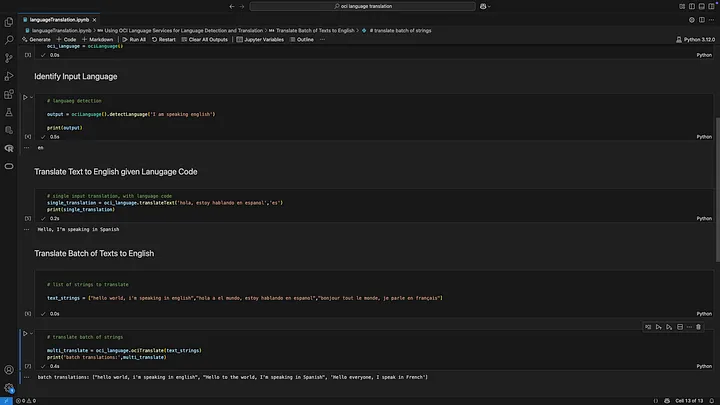
\includegraphics[width=0.9\textwidth]{Demo/Dich_nhieu_chuoi_van_ban.jpg}
    \caption{Thực hiện dịch nhiều chuỗi văn bản thông qua một lớp tùy chỉnh}
    \label{fig:cloud_intro}
\end{figure}

OCI Language Service là một dịch vụ API dễ sử dụng, cung cấp các mô hình ngôn ngữ đã được huấn luyện sẵn trên nền tảng OCI \cite{medium_exploring_oci_language_service}.

Sử dụng OCI Language Service, chúng ta có thể thực hiện các tác vụ sau:

\begin{myitem}
    \item Phát hiện ngôn ngữ (Language Detection)

    \item Phân loại văn bản (Text Classification)
    
    \item Phân tích cảm xúc (Sentiment Analysis)
    
    \item Trích xuất cụm từ khóa (Key Phrase Extraction)
    
    \item Nhận diện thực thể có tên (NER) (Named Entity Recognition)
    
    \item Phát hiện thông tin cá nhân (PII Detection)
    
    \item Xử lý ngôn ngữ tự nhiên trong lĩnh vực y tế (Healthcare NLP)
\end{myitem}

Dịch vụ này cũng cho phép chúng ta huấn luyện các mô hình tùy chỉnh để phân loại và nhận diện thực thể trên các bộ dữ liệu riêng của mình.

\subsubsection{Bắt đầu với OCI Python SDK}
OCI SDK cho Python cho phép chúng ta viết mã để quản lý các tài nguyên trên OCI cũng như gọi các dịch vụ đám mây như GenAI, Language, Vision, v.v.

Khi chạy mã trên máy tính cá nhân, chúng ta có thể dễ dàng thiết lập API key trong OCI Console, từ đó bắt đầu tương tác với các tài nguyên OCI thông qua SDK hoặc OCI CLI.

Để thiết lập API key, chúng ta thực hiện các bước sau:
\begin{myitem}
    \item Truy cập OCI Console.

    \item Vào mục My Profile trong Identity \& Security.
    
    \item Chọn Add API Key để thêm khóa API mới.
\end{myitem}

\begin{figure}[H] % cần gói float nếu muốn cố định vị trí
    \centering
    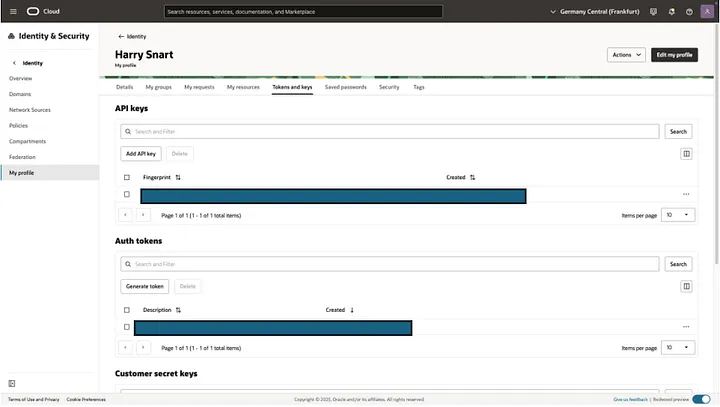
\includegraphics[width=0.9\textwidth, keepaspectratio]{Demo/Them_API_key (1).jpg}
    \caption{Thêm một API Key mới vào hồ sơ OCI}
    \label{fig:cloud_intro}
\end{figure}

Sau đó, hệ thống sẽ hỏi chúng ta muốn tạo mới hay tải lên một cặp khóa (key pair). Khi các khóa đã được tải xuống, chúng ta có thể thêm API Key mới vào hồ sơ OCI của mình.

\begin{figure}[H] % cần gói float nếu muốn cố định vị trí
    \centering
    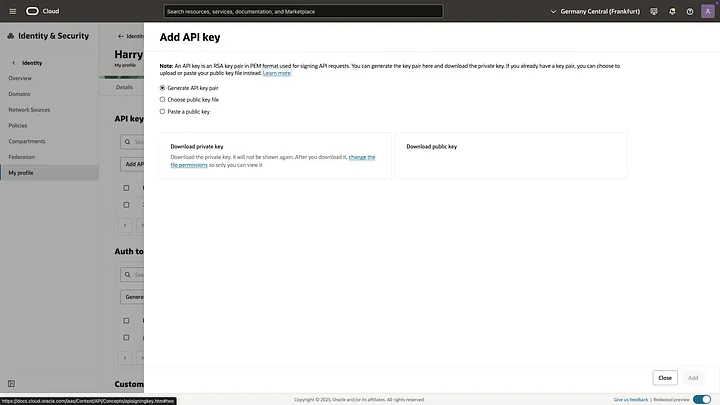
\includegraphics[width=0.9\textwidth, keepaspectratio]{Demo/Chon_cap_khoa.jpg}
    \caption{Chọn cặp khóa (key pair) cho API Key}
    \label{fig:cloud_intro}
\end{figure}

Hệ thống sẽ cung cấp cho chúng ta một mã nhận dạng duy nhất và tự động tạo một hồ sơ (profile).

\begin{figure}[H] % cần gói float nếu muốn cố định vị trí
    \centering
    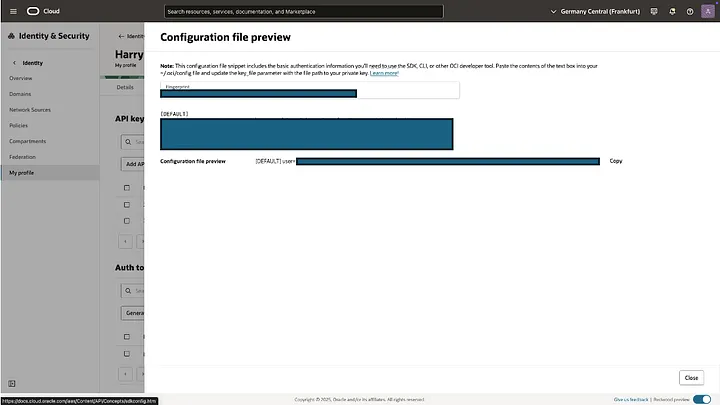
\includegraphics[width=0.95\textwidth, keepaspectratio]{Demo/Cau_hinh.jpg}
    \caption{Tạo tệp cấu hình cho API Key}
    \label{fig:cloud_intro}
\end{figure}

Theo mặc định, OCI SDK sẽ tìm tệp cấu hình tại:

\begin{center}
\fbox{\parbox{0.8\textwidth}{\texttt{~/.oci/config}}}
\end{center}

\textit{Lưu ý: nếu chúng ta có nhiều tenancy hoặc nhiều profile, chúng ta có thể thiết lập nhiều profile trong tệp cấu hình — chỉ cần đảm bảo không kết nối với profile DEFAULT khi sử dụng SDK.}

\subsubsection{Phát hiện ngôn ngữ (Language Detection)}
Chúng ta sẽ bắt đầu với API Phát hiện ngôn ngữ (Language Detection API). Dịch vụ này cho phép xử lý nhiều yêu cầu cùng lúc (batch), hỗ trợ phát hiện lên đến 100 bản ghi mỗi lần gọi API. API có thể nhận diện hơn 100 ngôn ngữ khác nhau.

Điều quan trọng cần lưu ý là mỗi lần gọi API chỉ trả về một ngôn ngữ chính. Nếu chúng ta gửi một batch chứa nhiều tài liệu đa ngôn ngữ, API sẽ trả về ngôn ngữ chiếm ưu thế trong batch đó.

Với OCI Python SDK, chúng ta có thể sử dụng các hàm trợ giúp (helper functions) để tạo payload đúng định dạng cho API theo phong cách Python, giúp việc gọi API trở nên thuận tiện và trực quan \cite{medium_exploring_oci_language_service}.

\begin{lstlisting}
# load python sdk for OCI
import oci

# instantiate an AI Client using config from profile
ai_client = oci.ai_language.AIServiceLanguageClient(oci.config.from_file())

# create function to detect input language
def detectLanguage(ai_client,text):
    ''' Detect language of input string, returning code '''
    doc1 = oci.ai_language.models.DominantLanguageDocument(key='key1', text=text)
    documents = [doc1]
    batch_detect_dominant_language_details = oci.ai_language.models.BatchDetectDominantLanguageDetails(documents=documents)
    output = ai_client.batch_detect_dominant_language(batch_detect_dominant_language_details)
    return output.data.documents[0].languages[0].code

# run function
detectLanguage("Hello world, I'm speaking English")

\end{lstlisting}

\subsubsection{Dịch ngôn ngữ (Language Translation)}
Để sử dụng API Dịch ngôn ngữ (Translation API), chúng ta có thể dùng SDK theo cách tương tự: chúng ta khởi tạo một client, sau đó sử dụng phương thức batch\_language\_translation.

Phương thức này cho phép chúng ta:
\begin{myitem}
    \item Đặt ngôn ngữ đầu vào cho từng tài liệu trong batch.

    \item Chọn ngôn ngữ đích mà chúng ta muốn dịch sang.

\end{myitem}

chúng ta có thể thực hiện dịch thời gian thực (real-time translation) hoặc dịch bất đồng bộ (asynchronous translation) cho các tệp lớn khi cần xử lý hàng loạt.

\begin{lstlisting}
# load python sdk for OCI
import oci

# instantiate an AI Client using config from profile
ai_client = oci.ai_language.AIServiceLanguageClient(oci.config.from_file())

# create function to translate text given language code    
def translateToEnglish(ai_client, input_text, language_code):
    ''' Translate text to English if not already English '''
    text_document =  oci.ai_language.models.TextDocument(
         key="1",
         text=input_text,
         language_code=language_code)
    
    try:
        # Run text classification on text_document
        text_translation = ai_client.batch_language_translation(
            batch_language_translation_details=oci.ai_language.models.BatchLanguageTranslationDetails(
                documents=[text_document],
                target_language_code="en"
            )
        )
        # return the data
        return text_translation.data.documents[0].translated_text


    # Print any API errors
    except Exception as e:
        print(e)
    return

# run function with sample string
translateToEnglish(ai_client,'hola, estoy hablando en espanol','es')

\end{lstlisting}

\subsubsection{Dịch đa ngôn ngữ theo batch (Batch Multi-Lingual Translation)}
Đối với dịch thời gian thực (real-time translation), việc kết hợp dịch vụ Phát hiện ngôn ngữ (Language Detection) và dịch vụ Dịch ngôn ngữ (Translation) khá đơn giản, cho phép tạo ra các bản dịch từ nhiều ngôn ngữ đầu vào khác nhau.

Ví dụ, đoạn code dưới đây có thể hữu ích như một bước tiền xử lý (pre-processing) cho Retrieval Augmented Generation (RAG) trên bộ sưu tập tài liệu đa ngôn ngữ, trước khi tiến hành chia nhỏ (chunking) và tách tài liệu.

\begin{lstlisting}
final_strings = []

for sentence in text_strings:
    language_code = detectLanguage(ai_client,sentence)
    
    if language_code != 'en':
        try:
            sentence = translateToEnglish(ai_client,sentence, language_code)
        except:
            print('language not supported!')
            sentence = 'language not supported for:'+sentence
    final_strings.append(sentence)

print('translated texts:', final_strings)

\end{lstlisting}

Cách làm này giúp chúng ta tạo ra bộ sưu tập tài liệu thống nhất về một ngôn ngữ, từ đó có thể sử dụng các mô hình embedding nhỏ hơn và hiệu quả hơn.

Để thuận tiện cho việc trình bày, đây là đoạn code gói gọn thành một lớp Python (Python class) nhằm minh họa cách các dịch vụ có thể hoạt động phối hợp với nhau.

\begin{lstlisting}
# load custom class
from ociLanguage import ociLanguage

# define OCI language client
oci_language = ociLanguage()

# list of strings to translate
text_strings = ["hello world, i'm speaking in english","hola a el mundo, estoy hablando en espanol","bonjour tout le monde, je parle en français"]

# translate batch of strings
multi_translate = oci_language.ociTranslate(text_strings)
print('batch translations:',multi_translate)

\end{lstlisting}

\newpage
\subsection*{\centering KẾT LUẬN CHƯƠNG 3}
\addcontentsline{toc}{subsection}{KẾT LUẬN CHƯƠNG 3}

Chương 3 đã cung cấp một cái nhìn tổng quan và chi tiết về dịch vụ điện toán đám mây của Oracle Cloud Infrastructure (OCI), từ việc tìm hiểu các loại dịch vụ chính (IaaS, PaaS, SaaS, DaaS) đến các quy trình đăng ký, đăng nhập và thử nghiệm thực tế với OCI Language Service. Qua các phân tích và thí nghiệm, có thể rút ra một số nhận định quan trọng như sau:

Trước hết, OCI nổi bật với hiệu năng cao, khả năng mở rộng linh hoạt và tính bảo mật vượt trội. Các tính năng như Autonomous Database, quản lý khóa và mã hóa dữ liệu, cùng với hệ thống IAM và Cloud Guard, đảm bảo dữ liệu của doanh nghiệp luôn được bảo vệ toàn diện. Đồng thời, cơ chế tự động hóa và hỗ trợ API giúp giảm thiểu khối lượng công việc vận hành, từ đó nâng cao hiệu quả triển khai và quản lý tài nguyên trên nền tảng đám mây.

Thứ hai, các dịch vụ thử nghiệm như OCI Language Service cho thấy khả năng ứng dụng thực tiễn của nền tảng trong lĩnh vực trí tuệ nhân tạo và xử lý ngôn ngữ tự nhiên. Việc tích hợp phát hiện ngôn ngữ, dịch thuật đa ngôn ngữ, phân loại văn bản và trích xuất thực thể cho thấy OCI không chỉ phục vụ nhu cầu hạ tầng mà còn cung cấp các giải pháp thông minh, hỗ trợ doanh nghiệp trong các nhiệm vụ phân tích dữ liệu và tự động hóa quy trình nghiệp vụ.

Bên cạnh các ưu điểm, chúng ta cũng nhận thấy một số hạn chế của Oracle Cloud, như chi phí tương đối cao đối với doanh nghiệp nhỏ, hệ sinh thái dịch vụ chưa rộng bằng các đối thủ lớn, và hạn chế về phạm vi trung tâm dữ liệu. Tuy nhiên, những nhược điểm này vẫn có thể được cân nhắc và quản lý thông qua lựa chọn gói dịch vụ phù hợp và tối ưu hóa quy trình triển khai.
